\section{A model of human behavior for \acl*{WCA}}\label{sec:model}

In~\cite{olguinmunoz:impact2021} we studied the effects of system responsiveness on human behavior in step-based \ac{WCA} through human-subject trials.
We employed a modified and instrumented version of the LEGO Assistant application devised by~\textcite{Chen2015LEGO}, which belongs to a category of \acp{WCA} with the goal of guiding a user through a sequential task.
The application monitors the progress of the task in ``realtime'' by repeatedly sampling the state of the physical system, most commonly through video frames.
Whenever the applications detects that the user has correctly or incorrectly performed an instruction, it provides a new instruction to either advance the task or correct the detected mistake.
Subjects interacted with this \ac{WCA} while the responsiveness of the system was altered in realtime and we captured key application and task performance metrics.
Additionally, we also employed questionnaires to evaluate key personality traits of the participants, and correlated these results to the task performance metrics collected.

From this experimentation, we identified four main results concerning the step execution times of humans in \ac{WCA}:

\begin{enumerate}
    \item System slow-down induces \emph{additional} behavioral slow-down which scales with the decrease in system responsiveness.
    Moreover, users become progressively slower the longer they spend in a degraded system state.

    \item The effects of system slow-down on human behavior remain for a while even after system responsiveness improves.
    
    \item Humans get faster at performing steps as the task progresses. However, this effect is dampened by reduced system responsiveness, even disappearing at higher levels of system impairment.
    
    \item The above effects seem to be modulated by the Big Five~\cite{oliver:bfi1999} trait of \emph{neuroticism}.
\end{enumerate}

In the following, we employ the above insights together with the actual data collected for~\cite{olguinmunoz:impact2021} to design and build a probabilistic model of human behavior for \ac{WCA}.
In order to accurately emulate the behavior of a human, such a model for needs to implement two main behaviors.
One, it needs to generate realistic \emph{execution times} for each step in the task, considering the current and historical impairment of the \ac{WCA} system.
And two, it needs to produce sequences of video frames for each step which mimic what a human generate.

\subsection{Generating realistic timings}

We begin by providing some definitions relating to step-based \acl{WCA}.
First of all, a \emph{step} is understood as a specific action to be performed by the user, described by a single instruction; a \emph{task} consists of a series of steps to be executed in sequence (see \cref{fig:task}).
More formally, a step starts when the corresponding instruction is provided to the user, and ends when the instruction for the next step is provided.
We call the time interval between these two events the \emph{step duration}.

Take \( \{ t_0, t_1, \ldots, t_{n + 1} \} \) a series of discrete and sequential sampling intervals at which the \ac{WCA} captures the state of the physical system --- see \cref{fig:step}.
\( t_0 \) corresponds to the instant at which the instruction for step \( M \) is provided and the first sample for said step is taken, and \( t_{n+1} \) to the instant at which the instruction for step \( M + 1 \) is provided.
Furthermore, \( t_c \) represents the instant at which the user finishes performing the instruction for step \( M \); the interval \( t_c - t_0 \) we call the \emph{execution time} of \( M \).
From the discrete sampling nature of the \ac{WCA} application, it follows that \( t_{n - 1} \leq t_c \leq t_{n} \); in plain English, the final state of the step is --- by definition --- always reached \emph{before} the final sample of the step is taken but after the next-to-last sampling instant.
We define the intervals \( t_n - t_c \) and \( t_{n + 1} - t_n \) as the \emph{wait time} and \emph{last sample \ac{RTT}}, respectively, for step \( M \).
The sum of these two values (i.e. the interval \( t_{n + 1} - t_c \)) we call \emph{time-to-feedback}.

\emph{Execution time} and \emph{time-to-feedback} correspond to the two key metrics necessary to characterize the interactions between human behavior and system responsiveness.

\begin{figure}
    \centering
    \begin{subfigure}{\columnwidth}
        \centering
        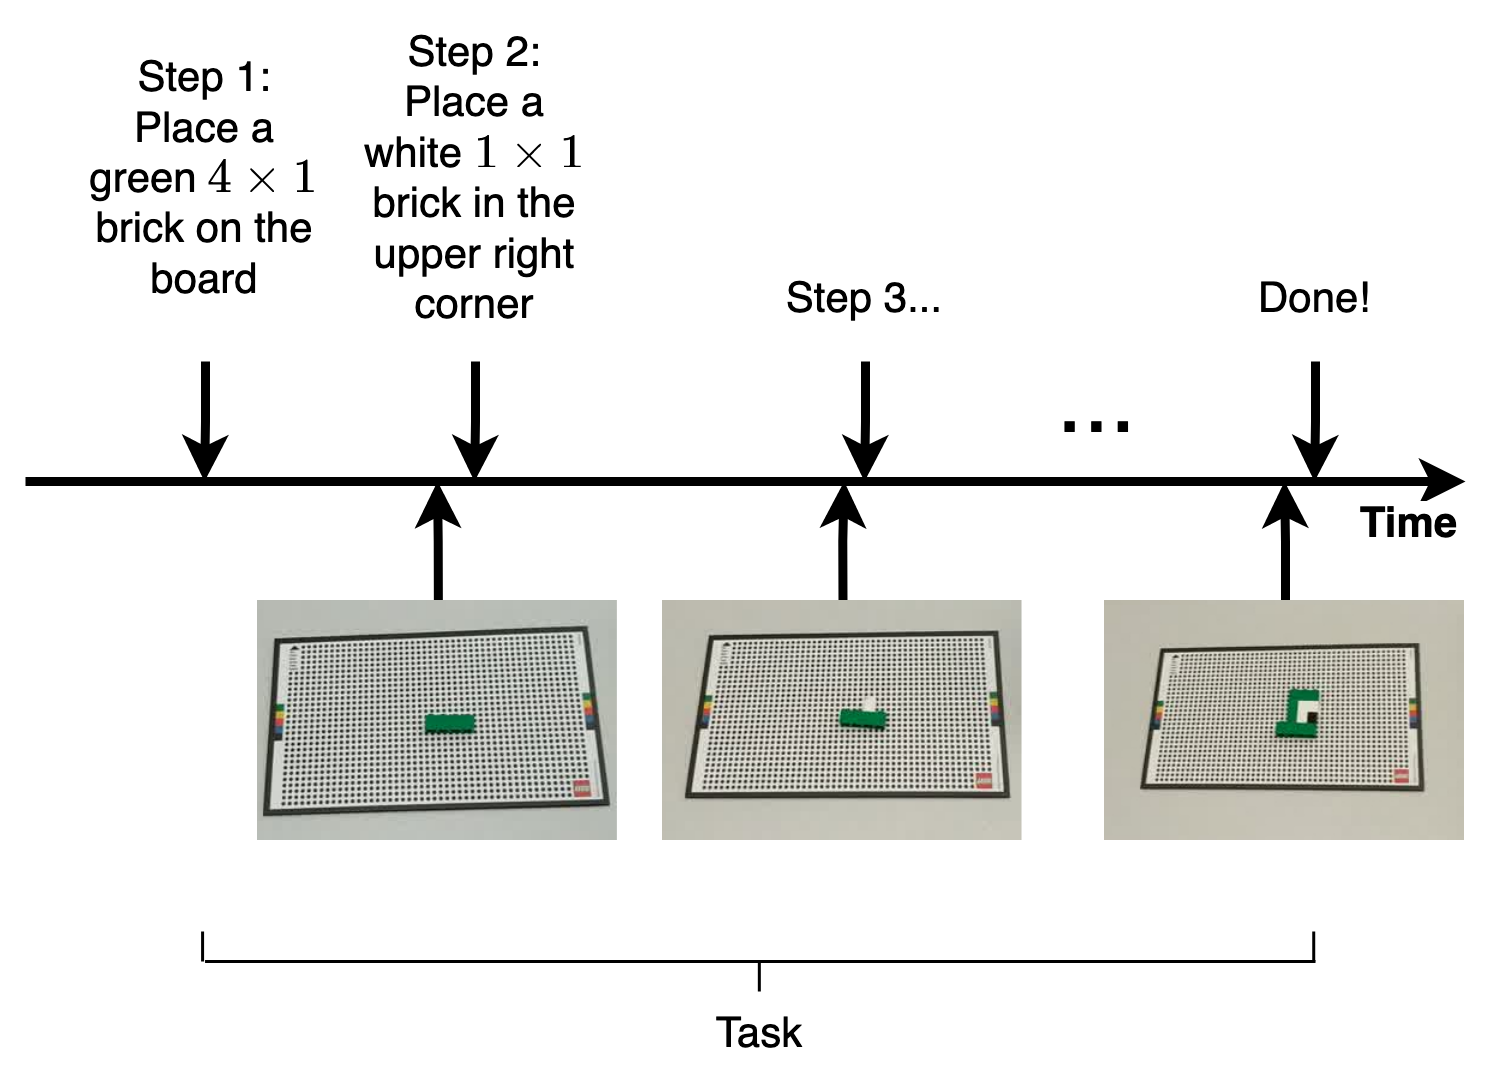
\includegraphics[width=\columnwidth]{figs/task.png}
        \caption{%
            Overview of a task in a \ac{WCA}, composed of a series of steps.
            Each steps starts with an instruction being provided to the user and ends with the instruction for the next step.
            The \ac{WCA} continuously samples the task state, automatically triggering transitions between steps as correct (or incorrect) states are recognized.
        }\label{fig:task}
    \end{subfigure}\\
    \begin{subfigure}{\columnwidth}
        \centering
        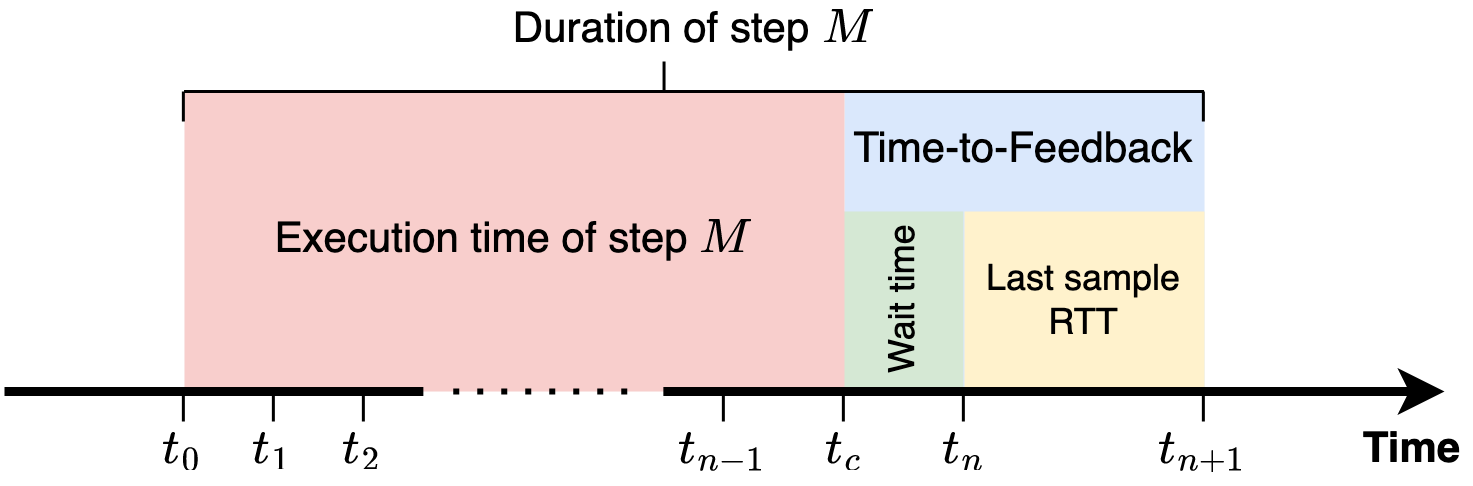
\includegraphics[width=\columnwidth]{figs/step_time.png}
        \caption{%
            Breakdown of a step into its timing components.
            The instruction for step \( M \) and \( M + 1 \) are provided to the user at \( t_0 \) and \( t_{n+1} \), respectively.
            \( t_k | k \in \{1, \ldots, n \} \) correspond to the \ac{WCA} sampling instants for step \( M \), and \( t_c \) marks the instant at which the user finishes performing the instruction.
        }\label{fig:step}
    \end{subfigure}
    \caption{}
\end{figure}

\todo[inline]{Diagram of model?}

\begin{algorithm}
    \caption{Timing model algorithm}
    \KwIn{%
        \begin{itemize}
            \item $T_\text{start}$: start timestamp of the previous step.
            \item $T_\text{success}$: capture timestamp of the succesful sample of the previous step.
            \item $T_\text{end}$: end timestamp of the previous step.
            \item $t_\text{exec}$: execution time (in seconds) of the previous step.
        \end{itemize}%
    }
    \KwOut{$t_\text{exec}'$: execution time for the current step.}

    \Comment{%
        Initial values:\\
        $d \leftarrow 0$\\
        $I_\text{prev} \leftarrow \text{NULL}$
    }
    $t_\text{wait} \leftarrow T_\text{success} - (T_\text{start} + t_\text{exec})$\;
    $t_\text{round-trip} \leftarrow T_\text{end} - T_\text{success}$\;
    $i \leftarrow t_\text{wait} + t_\text{round-trip}$ \Comment*[r]{raw impairment}
    $I \leftarrow \text{BIN}(i)$ \Comment*[r]{bin impairment into\\discrete levels}

    \If{$I_\text{prev} == \text{NULL}$}{%
        $d \leftarrow 1$\;
        $T \leftarrow \text{NO TRANSITION}$\;
    } \ElseIf{$I_\text{prev} < I$}{%
        $d \leftarrow 1$\;
        $T \leftarrow \text{LOWER TO HIGHER} $
    } \ElseIf{$I_\text{prev} > I$}{%
        $d \leftarrow 1$\;
        $T \leftarrow \text{HIGHER TO LOWER} $  
    }

\end{algorithm}


This data is first preprocessed and then sampled according to a series of rules in order to produce novel,realistic sequences of execution times for a task.
Alternatively, instead of sampling directly from the preprocessed data, a theoretical distribution can be fitted, thus allowing for generation of realistic synthetic execution times.

\subsubsection{Data pre-processing}

A sample of the step timing data obtained for~\cite{olguinmunoz:impact2021} is presented in \cref{tab:exec_times:empirical}.
This data corresponds to real step execution times for \num{40} repetitions, by different human subjects, of the same \num{169}-step task.
During each repetition of the task, system responsiveness was altered in real time by setting the round-trip-times of all frames to a fixed value (corresponding to the \emph{delay} column in \cref{tab:exec_times:empirical}).
For more details on the experimental design and data collection procedure, please see the original article~\cite{olguinmunoz:impact2021}.

We process this data in the following manner:

\begin{table*}
    \centering
    \caption{}\label{tab:exectime:proc}
\begin{tabular}{rrrllll}
\toprule
subject ID &  step &  next exec. time & neuroticism &  impairment & transition tag & duration \\
\midrule
\num{136516} &   \num{67} & \SI{4.663}{\second} & medium & high & no transition & short \\
%
\num{137299} &  \num{114} & \SI{2.230}{\second} & low & low & higher-to-lower &  short \\
\num{137344} &   \num{45} & \SI{1.775}{\second} & low &  medium & no transition & medium \\
\num{135955} &   \num{77} & \SI{4.326}{\second} & low &  high & no transition & long \\
\num{135385} &  \num{129} & \SI{2.499}{\second} & high &  medium & no transition & long \\
\bottomrule
\end{tabular}
\todo[inline]{Use same samples as first table for clarity!}
\end{table*}
    

\begin{enumerate}
    \item Normalized neuroticism values are binned into predefined, contiguous bins.
    We use three bins with edges
    \( \left(-\infty, \frac{1}{3}\right) \),
    \( \left[\frac{1}{3}, \frac{2}{3}\right) \),
    and \( \left[\frac{2}{3}, \infty\right) \),
    as these give the most even distribution of number of samples across bins.

    \item System impairment (\emph{delay}) is binned into predefined, contiguous bins.
    Once again, we use three bins giving a somewhat even distribution of samples:
    \( \left(-\infty, 1.0\right) \),
    \( \left[1.0, 2.0\right) \),
    and \( \left[2.0, \infty\right) \) seconds.

    \item A predefined number of steps (by default, \num{8}) immediately after each change in binned impairment are marked according to the relative change in impairment: \emph{low-to-high}, or \emph{high-to-low} impairment.
    We label this value the \emph{transition tag}.
    Steps at the beginning of the task (where there is no previous impairment), or too far away from a transition in impairment, are tagged as \emph{no transition}.

    \item Each step in a sequence tagged with the same transition tag is assigned a sequential \emph{duration} number.
    This value tracks how long the system has been in a specific state, and is in turn binned into three bins:
    \( \left[0, 5\right) \),
    \( \left[5, 10\right) \),
    and \( \left[10, \infty\right) \) steps.

    \item Finally, execution times are shifted by one step.
    This is because the execution time of a step depends on the state of the previous step, and not the current one.
    As explained previously, humans only becomes aware of the responsiveness of the system when they finish a step and have to wait for feedback from the system.
\end{enumerate}


\subsection{Generating a synthetic trace of frames}

\subsection{Model implementation}

The model is provided as a Python~\num{3.10} library which includes \acp{API} for the generation of realistic execution times and synthetic traces of video frames.

\subsection{Verifying the model}